\documentclass{beamer}
\usepackage{tikz}
\usepackage{drawstack}

\usetikzlibrary{graphs,quotes,arrows,automata}

\mode<presentation>
\usefonttheme{serif}

\beamertemplatenavigationsymbolsempty
\setbeamertemplate{footline}[frame number]

\definecolor{lightred}{rgb}{0.8,0.8,1}
\definecolor{lightgrey}{rgb}{0.8,0.8,0.8}

\title{}
\author{Martin \textsc{Vassor}}

\institute[\'Ecole polytechnique f\'ed\'erale de Lausanne] 
{
  DSLab, EPFL
  \vspace{0.5cm}

  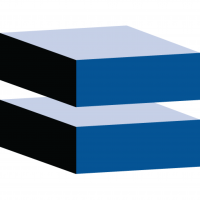
\includegraphics[height=1cm]{DSLab.png}
  \hspace{0.1cm}
  
\includegraphics[height=1cm]{epfl.eps}
}


\newcommand{\keyvalue}[2] {
		\begin{tabular}{|c|c|}
			\hline
			\texttt{#1} & \texttt{#2} \\
			\hline
		\end{tabular}
}

\begin{document}

\subject{Verified double-hashed hash table}
\AtBeginSection[] {
  \begin{frame}<beamer>{Outline}
    \tableofcontents[currentsection,currentsubsection]
  \end{frame}
} 

\begin{frame}
\titlepage
\end{frame}

\section{Introduction}
\begin{frame}
	\frametitle{Naive hash table}
	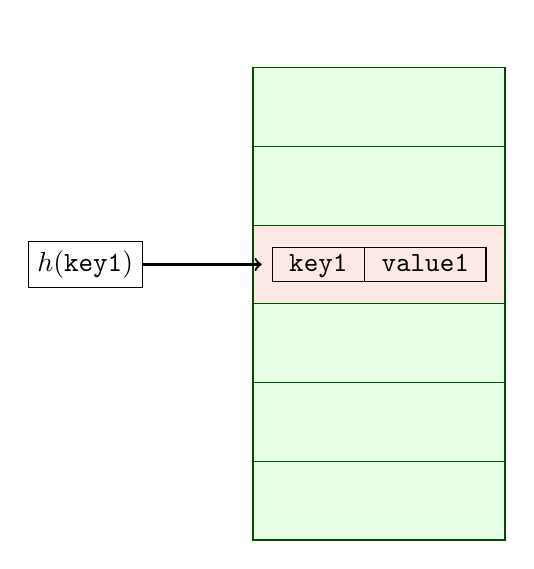
\begin{tikzpicture}
		\draw (0, -3) node[draw, anchor=east] (key1) {$h(\mathtt{key1})$};

		\drawstruct{(3,0)}
		\structcell[freecell]{} \coordinate(firstCell) at (currentcell.east) ;
		\structcell[freecell]{} \coordinate(secondCell) at (currentcell.east);
		\structcell[occupiedcell]{\keyvalue{key1}{value1}} \coordinate(thirdCell) at (currentcell.west);
		\structcell[freecell]{} \coordinate(fourthCell) at (currentcell.east);
		\structcell[freecell]{} \coordinate(fifthCell) at (currentcell.east);
		\structcell[freecell]{} \coordinate(sixthCell) at (currentcell.east);

		\draw[->, thick] (key1) -- (thirdCell);
	\end{tikzpicture}

\end{frame}

\begin{frame}
	\frametitle{Naive hash table}
	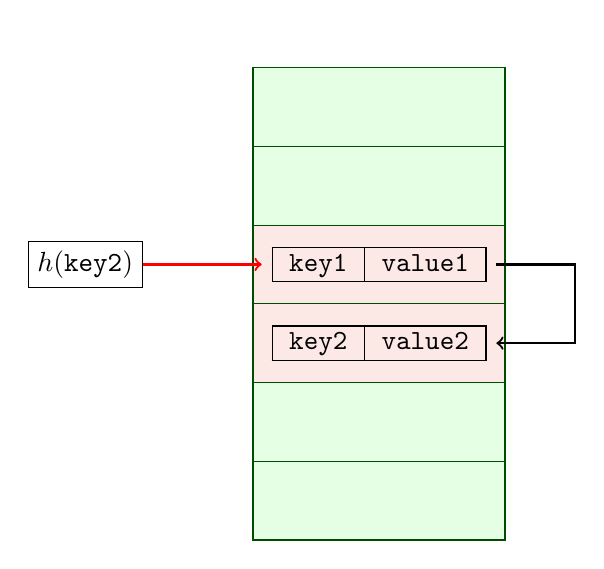
\begin{tikzpicture}
		\draw (0, -3) node[draw, anchor=east] (key2) {$h(\mathtt{key2})$};

		\drawstruct{(3,0)}
		\structcell[freecell]{} \coordinate(firstCell) at (currentcell.east) ;
		\structcell[freecell]{} \coordinate(secondCell) at (currentcell.east);
		\structcell[occupiedcell]{\keyvalue{key1}{value1}} \coordinate(thirdCell) at (currentcell.west); \coordinate(thirdCellOut) at (currentcell.east);
		\structcell[occupiedcell]{\keyvalue{key2}{value2}} \coordinate(fourthCell) at (currentcell.east); \coordinate(fourthCellOut) at (currentcell.east);
		\structcell[freecell]{} \coordinate(fifthCell) at (currentcell.east);
		\structcell[freecell]{} \coordinate(sixthCell) at (currentcell.east);

		\draw[->, red, thick] (key2) -- (thirdCell);
		\draw[->, thick] (thirdCellOut) -- ++(1, 0) |- (fourthCellOut);
	\end{tikzpicture}
\end{frame}

\begin{frame}
	\frametitle{Naive hash table}
	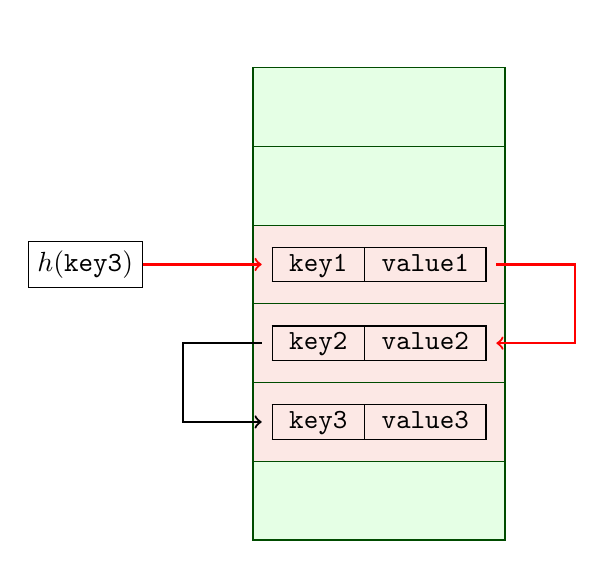
\begin{tikzpicture}
		\draw (0, -3) node[draw, anchor=east] (key3) {$h(\mathtt{key3})$};

		\drawstruct{(3,0)}
		\structcell[freecell]{} \coordinate(firstCell) at (currentcell.east) ;
		\structcell[freecell]{} \coordinate(secondCell) at (currentcell.east);
		\structcell[occupiedcell]{\keyvalue{key1}{value1}} \coordinate(thirdCell) at (currentcell.west); \coordinate(thirdCellOut) at (currentcell.east);
		\structcell[occupiedcell]{\keyvalue{key2}{value2}} \coordinate(fourthCell) at (currentcell.west); \coordinate(fourthCellOut) at (currentcell.east);
		\structcell[occupiedcell]{\keyvalue{key3}{value3}} \coordinate(fifthCell) at (currentcell.west); \coordinate(fifthCellOut) at (currentcell.east);
		\structcell[freecell]{} \coordinate(sixthCell) at (currentcell.east);

		\draw[->, red, thick] (key3) -- (thirdCell);
		\draw[->, red, thick] (thirdCellOut) -- ++(1, 0) |- (fourthCellOut);
		\draw[->, thick] (fourthCell) -- ++(-1, 0) |- (fifthCell);
	\end{tikzpicture}
\end{frame}

\begin{frame}
	\frametitle{Double hashing}
\end{frame}

\begin{frame}
	\frametitle{Provided implementation}
\end{frame}

\begin{frame}
	\frametitle{Provided verification}
\end{frame}

\section{Implementation}
\subsection{Modifications}
\subsection{Performance evaluation}
\subsection{Performance results}


\section{Verification}
\subsection{What to prove ?}
\subsection{Proof steps}


\section{Conclusion}
\subsection{Hash Table software}
\begin{frame}
	\frametitle{Hash-Table software}
	\begin{itemize}
		\item Efficient (when key is present).
		\item Formally verified.
		\item Requires \texttt{capacity} and \texttt{offset} coprime.
	\end{itemize}
\end{frame}

\subsection{Side effects}
\begin{frame}
	\frametitle{Side effects}
	\begin{itemize}
		\item 6 commits in Verifast tree (\texttt{long long} support).
		\item 9 issues on Verifast.
		\item A random access sequence generator \& benchmark.
	\end{itemize}
\end{frame}



\begin{frame}
\begin{center}
\huge{Q\&A}
\end{center}
\end{frame}

\end{document}
